\documentclass[12pt,a4paper]{article}

% ---------- Packages ----------
\usepackage[utf8]{inputenc}
\usepackage[T1]{fontenc}
\usepackage{lmodern}
\usepackage[french]{babel}
\usepackage[margin=2.5cm]{geometry}
\usepackage{booktabs}
\usepackage{tabularx}
\usepackage{array}
\usepackage{graphicx}
\usepackage{float}
\usepackage{amsmath}
\usepackage{enumitem}
\usepackage{xcolor}
\usepackage{setspace}
\usepackage{fancyhdr}
\usepackage[hidelinks]{hyperref}

\setstretch{1.15}
\setlength{\headheight}{15pt}
\setlength{\parindent}{0pt}
\setlength{\parskip}{0.6em}

% En-tête / pied de page
\pagestyle{fancy}
\fancyhf{}
\lhead{SmartFactory AI}
\rhead{Master 2 Data Science}
\cfoot{\thepage}

\begin{document}

% ---------- Page de titre ----------
\begin{titlepage}
\centering
\vspace*{1.5cm}
{\large Master 2 Data Science\par}
{\large Matière : Analyse Python\par}
\vspace{2.5cm}
{\Huge\bfseries SmartFactory AI\par}
\vspace{0.6cm}
{\Large Système intelligent de détection d'anomalies\\
et de prédiction des pannes industrielles\par}
\vspace{3cm}
\begin{tabular}{rl}
\textbf{Réalisé par :} & Ghita Snoussi \\
\textbf{Encadrant :} & Non renseigné \\
\textbf{Année universitaire :} & 2026--2027 \\
\end{tabular}
\vfill
{\large \today\par}
\end{titlepage}

% ---------- Remerciements ----------
\section*{Remerciements}
\addcontentsline{toc}{section}{Remerciements}
Je remercie l'équipe pédagogique du Master 2 Data Science pour l'accompagnement méthodologique fourni dans le cadre de ce projet. Je remercie également les personnes qui ont contribué à la mise à disposition du jeu de données AI4I~2020 et à la documentation des outils Python utilisés. Ce texte peut être personnalisé avant le dépôt final.

% ---------- Résumé ----------
\begin{abstract}
Ce projet porte sur la maintenance prédictive dans le contexte de l'Industrie~4.0. À partir du jeu de données AI4I~2020 (10\,000 observations de machines industrielles), nous construisons un pipeline complet de Machine Learning : prétraitement, analyse exploratoire, réduction de dimension par PCA, regroupement par K-Means, puis classification supervisée avec six algorithmes (régression logistique, KNN, SVM, arbre de décision, Random Forest et Gradient Boosting). Les modèles sont comparés avec les variables originales et avec les composantes principales, à l'aide de métriques adaptées au déséquilibre des classes (Recall, F1-score, PR-AUC). Le Random Forest optimisé atteint sur le test une précision de 0,903, un recall de 0,824, un F1-score de 0,862 et une PR-AUC de 0,882. Les variables mécaniques, thermiques et liées à l'usure expliquent l'essentiel du signal prédictif, tandis que la PCA dégrade les performances de classification.

\medskip
\textbf{Mots-clés :} maintenance prédictive, détection d'anomalies, PCA, K-Means, classification, déséquilibre de classes, Random Forest.
\end{abstract}

\section*{Abstract}
\addcontentsline{toc}{section}{Abstract}
This project addresses predictive maintenance in the context of Industry~4.0. Based on the AI4I~2020 dataset, a complete data science pipeline was implemented: data preparation, exploratory analysis, principal component analysis, K-Means clustering, supervised classification and model interpretation. Six classifiers were compared using the original variables and principal components, with metrics suited to rare failures. The optimized Random Forest achieved a precision of 0.903, a recall of 0.824, an F1-score of 0.862 and a PR-AUC of 0.882 on the test set. The Streamlit dashboard connects the saved artifacts to an interactive environment for sensor exploration, anomaly screening and machine-level predictions. The results remain exploratory because the dataset is synthetic and has no temporal dimension.

\medskip
\textbf{Keywords:} predictive maintenance, industrial anomaly detection, PCA, K-Means, imbalanced classification, Random Forest, Streamlit.

\tableofcontents
\listoffigures
\listoftables
\section*{Liste des abréviations}
\addcontentsline{toc}{section}{Liste des abréviations}
\begin{tabularx}{\textwidth}{@{}l X@{}}
\textbf{AI4I} & Artificial Intelligence for Industry \\
\textbf{EDA} & Exploratory Data Analysis, ou analyse exploratoire des données \\
\textbf{PCA} & Principal Component Analysis, ou analyse en composantes principales \\
\textbf{KPI} & Key Performance Indicator, ou indicateur clé de performance \\
\textbf{MDI} & Mean Decrease in Impurity, importance par diminution d'impureté \\
\textbf{ROC-AUC} & Aire sous la courbe Receiver Operating Characteristic \\
\textbf{PR-AUC} & Aire sous la courbe Precision--Recall \\
\textbf{TWF/HDF/PWF/OSF/RNF} & Modes de panne fournis par AI4I~2020 \\
\end{tabularx}
\newpage

% =====================================================
\section{Chapitre 1 — Introduction générale}

\subsection{Contexte}
Dans l'Industrie~4.0, les machines sont équipées de capteurs qui mesurent en continu des grandeurs physiques (température, vitesse de rotation, couple, usure, etc.). Ces données permettent de détecter des comportements anormaux et d'anticiper les défaillances, afin de réduire les arrêts imprévus et d'optimiser la maintenance. Une panne non anticipée coûte généralement plus cher qu'une intervention préventive, d'où l'intérêt des approches prédictives.

\subsection{Problématique}
Comment exploiter les données issues des capteurs industriels pour détecter automatiquement les comportements anormaux, prédire les défaillances des machines et identifier les facteurs les plus associés aux pannes ?

\subsection{Objectifs}
L'objectif général est de développer un prototype de système de maintenance prédictive. Les objectifs spécifiques sont les suivants :
\begin{itemize}[noitemsep]
  \item préparer et explorer les données des capteurs ;
  \item réduire la dimensionnalité avec la PCA et visualiser les observations ;
  \item identifier des groupes de comportements avec K-Means et rechercher des machines atypiques ;
  \item comparer plusieurs algorithmes de classification, avec et sans PCA ;
  \item identifier les variables les plus influentes ;
  \item proposer une application interactive avec Streamlit.
\end{itemize}

\subsection{Organisation du rapport}
La section~\ref{sec:donnees} présente les données. La section~\ref{sec:methodo} décrit la méthodologie. Les sections~\ref{sec:resultats} à~\ref{sec:interpretation} exposent les résultats, discutés en section~\ref{sec:discussion}. La section~\ref{sec:app} présente l'application et la section~\ref{sec:conclusion} conclut le rapport après l'analyse des limites et perspectives.

% =====================================================
\section{Chapitre 2 — Fondements théoriques}\label{sec:theorie}

\subsection{Data Science et maintenance prédictive}
La Data Science industrielle combine l'acquisition de mesures, la statistique, l'apprentissage automatique et la restitution des résultats. Dans une démarche de maintenance prédictive, l'objectif n'est pas seulement de décrire l'état courant d'une machine, mais d'estimer le risque d'une défaillance afin d'organiser une intervention avant l'arrêt. Cette démarche complète la maintenance corrective, déclenchée après panne, et la maintenance préventive systématique, planifiée selon un calendrier fixe. Elle peut réduire les arrêts non planifiés, mais exige une validation attentive des faux négatifs, des fausses alertes et de la stabilité des capteurs.

\subsection{Analyse exploratoire et qualité des données}
L'EDA vise à comprendre la structure des observations avant tout apprentissage : types, valeurs manquantes, doublons, distributions, dépendances et déséquilibre de la cible. Une corrélation linéaire élevée ne prouve pas une relation causale et une faible corrélation n'exclut pas une relation à seuil. C'est pourquoi l'analyse combine statistiques, visualisations et connaissance du procédé industriel.

\subsection{Valeurs aberrantes et standardisation}
Pour une variable $x$, la règle de l'intervalle interquartile identifie comme atypiques les valeurs situées hors de
\[
[Q_1-1{,}5\,IQR,\;Q_3+1{,}5\,IQR],\qquad IQR=Q_3-Q_1.
\]
Dans un contexte de panne, une valeur extrême peut être un signal utile plutôt qu'une erreur de mesure. La standardisation utilisée dans ce projet est
\[
z_i=\frac{x_i-\mu_{\mathrm{train}}}{\sigma_{\mathrm{train}}},
\]
où $\mu_{\mathrm{train}}$ et $\sigma_{\mathrm{train}}$ sont estimés uniquement sur l'apprentissage. Cette précaution évite de transmettre au modèle une information calculée sur le test.

\subsection{Feature engineering}
L'ingénierie des caractéristiques traduit des relations métier en variables exploitables. Ici, l'écart de température renseigne sur la dissipation thermique, la puissance mécanique est calculée par $P=C\omega$ avec $\omega=2\pi n/60$, et le produit couple--usure représente une sollicitation cumulée. Ces transformations rendent explicites des interactions qui seraient plus difficiles à apprendre avec un modèle linéaire.

\subsection{PCA}
La PCA cherche des directions orthogonales maximisant la variance projetée. Si $X$ est la matrice standardisée, les composantes sont obtenues à partir des vecteurs propres de la matrice de covariance $X^\top X$. La variance expliquée par la composante $j$ vaut $\lambda_j/\sum_k\lambda_k$, où $\lambda_j$ est la valeur propre associée. La PCA est utile pour visualiser et compresser, mais l'optimisation de variance n'est pas équivalente à l'optimisation de la séparation des pannes.

\subsection{K-Means et détection d'anomalies}
K-Means alterne l'affectation de chaque observation au centroïde le plus proche et la mise à jour des centroïdes. Il minimise l'inertie
\[
J=\sum_{j=1}^{k}\sum_{x_i\in C_j}\lVert x_i-\mu_j\rVert^2.
\]
Le score de silhouette compare la cohésion d'un point dans son cluster à sa séparation d'avec les autres clusters. Après apprentissage, la distance au centroïde le plus proche peut constituer un score d'anomalie. Un percentile élevé augmente la précision mais diminue généralement le recall.

\subsection{Classification et déséquilibre}
La classification supervisée apprend une fonction séparant la classe normale de la classe panne. La régression logistique modélise une probabilité par une fonction sigmoïde ; KNN utilise la proximité des observations ; le SVM cherche une frontière à marge maximale ; les arbres construisent des règles ; les forêts agrègent des arbres randomisés ; le gradient boosting corrige séquentiellement les erreurs. Les poids de classe équilibrés sont utilisés par plusieurs modèles pour éviter que la classe majoritaire domine l'objectif.

\subsection{Métriques et interprétabilité}
Pour une matrice de confusion, la precision $VP/(VP+FP)$ mesure la fiabilité des alertes, tandis que le recall $VP/(VP+FN)$ mesure la capacité à ne pas manquer les pannes. Le F1 est leur moyenne harmonique. Lorsque la panne est rare, la PR-AUC est souvent plus informative que l'accuracy ou la ROC-AUC. L'interprétabilité est abordée ici par l'importance MDI, la permutation et les groupes de variables. Ces méthodes décrivent l'association entre variables et performance ; elles ne constituent pas une preuve de causalité.

% =====================================================
\section{Chapitre 3 — Présentation du jeu de données et analyse exploratoire}\label{sec:donnees}

\subsection{Source}
Le jeu de données utilisé est \emph{AI4I 2020 Predictive Maintenance}, publié par Matzka (2020) et disponible sur le dépôt UCI Machine Learning Repository. Il contient 10\,000 observations et 14 variables. Il s'agit de \textbf{données synthétiques} qui reproduisent le comportement d'une machine de fabrication, et non de mesures issues d'une usine réelle.

\subsection{Description des variables}

\begin{table}[H]
\centering
\small
\begin{tabularx}{\textwidth}{@{}l l X@{}}
\toprule
\textbf{Variable} & \textbf{Type} & \textbf{Description} \\
\midrule
UDI & Identifiant & Numéro de ligne (1 à 10\,000) \\
Product ID & Identifiant & Référence du produit \\
Type & Catégorielle & Qualité du produit : L (faible, $\approx$60\,\%), M (moyenne, $\approx$30\,\%), H (haute, $\approx$10\,\%) \\
Air temperature [K] & Numérique & Température de l'air ambiant \\
Process temperature [K] & Numérique & Température du processus \\
Rotational speed [rpm] & Numérique & Vitesse de rotation \\
Torque [Nm] & Numérique & Couple \\
Tool wear [min] & Numérique & Usure de l'outil \\
Machine failure & Binaire (cible) & 1 si la machine est en panne \\
TWF, HDF, PWF, OSF, RNF & Binaires & Modes de panne : usure de l'outil, dissipation thermique, puissance, surcharge, panne aléatoire \\
\bottomrule
\end{tabularx}
\caption{Variables du jeu de données AI4I 2020.}
\end{table}

\subsection{Déséquilibre des classes}
La classe « panne » est minoritaire : 339 observations sur 10\,000 (3,39\,\%), contre 9\,661 machines normales. Le jeu d'apprentissage contient 271 pannes sur 8\,000 lignes (3,39\,%) et le test 68 pannes sur 2\,000 lignes (3,40\,%). Ce déséquilibre a des conséquences majeures sur le choix des métriques et des méthodes, détaillées en section~\ref{sec:methodo}.

\subsection{Écart avec l'énoncé}
L'énoncé mentionne des capteurs de vibration, de pression, de tension et de courant. Le jeu de données ne contient que la température, la vitesse de rotation, le couple et l'usure. L'étude porte donc sur ces variables.

% =====================================================
\section{Chapitre 4 — Prétraitement et méthodologie}\label{sec:methodo}

Le pipeline suit l'ordre : données brutes, prétraitement, exploration, réduction de dimension, apprentissage non supervisé, classification, évaluation, interprétation, application. Tout le code est réalisé en Python (Pandas, NumPy, Scikit-learn, Matplotlib, Seaborn) dans des notebooks Jupyter.

\subsection{Prétraitement}

\paragraph{Qualité des données.} Le fichier nettoyé contient 10\,000 lignes et 18 colonnes après création des variables dérivées. La vérification ne révèle aucune valeur manquante ni doublon.

\paragraph{Valeurs aberrantes.} Elles ont été détectées avec la règle de l'IQR (valeurs situées au-delà de $Q_1 - 1{,}5\times \mathrm{IQR}$ ou de $Q_3 + 1{,}5\times \mathrm{IQR}$). Aucun outlier n'est détecté pour les températures et l'usure, contre 418 pour la vitesse de rotation et 69 pour le couple. Les lignes présentant un outlier ont un taux de panne de 15,69\,\%, contre 2,80\,\% pour les autres. Nous avons \textbf{conservé} ces valeurs, car les conditions extrêmes sont précisément susceptibles de précéder une défaillance.

\paragraph{Fuite de données (\emph{data leakage}).} Les colonnes TWF, HDF, PWF, OSF et RNF sont les causes directes de la panne : \texttt{Machine failure} vaut 1 dès qu'une d'elles vaut 1. Les utiliser comme variables explicatives donnerait des performances artificielles proches de 100\,\%. Elles ont donc été exclues des variables d'entrée. Les identifiants UDI et Product ID, sans valeur prédictive, ont aussi été retirés.

\paragraph{Encodage.} La variable \texttt{Type} a été encodée de manière ordinale (L\,=\,0, M\,=\,1, H\,=\,2), qui correspond à l'ordre naturel de qualité.

\paragraph{Séparation et normalisation.} Les données sont séparées en 80\,\% d'apprentissage et 20\,\% de test, avec une \textbf{stratification} sur la cible pour conserver la même proportion de pannes dans les deux ensembles. La normalisation (\texttt{StandardScaler} : moyenne 0, écart-type 1) est ajustée \textbf{uniquement sur l'ensemble d'apprentissage}, puis appliquée au test, pour éviter toute fuite d'information. Elle est indispensable pour la PCA, K-Means, KNN et SVM, qui reposent sur des distances et sont sensibles aux échelles (la vitesse, $\approx$1\,500, écraserait la température, $\approx$300).

\subsection{Feature engineering}
Trois variables ont été construites à partir de la physique du système :

\begin{table}[H]
\centering
\small
\begin{tabularx}{\textwidth}{@{}l X X@{}}
\toprule
\textbf{Variable} & \textbf{Formule} & \textbf{Lien avec les pannes} \\
\midrule
\texttt{Temp\_diff} & Température du processus $-$ température de l'air & Dissipation thermique (HDF) \\
\texttt{Power} & Couple $\times$ vitesse angulaire ($2\pi \times \text{rpm}/60$), en watts & Puissance (PWF) \\
\texttt{Torque\_x\_Wear} & Couple $\times$ usure de l'outil & Surcharge (OSF) \\
\bottomrule
\end{tabularx}
\caption{Variables construites par feature engineering.}
\end{table}

\subsection{Analyse exploratoire}
L'analyse comprend les statistiques descriptives, les distributions des variables selon l'état de la machine, les boxplots par classe, le taux de pannes par type de produit, la matrice de corrélation et la distribution des variables par mode de panne. Les résultats sont présentés en section~\ref{sec:eda}.

\subsection{Réduction de dimension : PCA}
La PCA (\emph{Principal Component Analysis}) transforme les variables corrélées en composantes principales orthogonales, classées par variance expliquée décroissante. Elle est ajustée sur l'ensemble d'apprentissage. Le nombre de composantes retenues est choisi pour conserver 95\,\% de la variance, à l'aide du scree plot et de la variance cumulée. Les loadings et le cercle des corrélations servent à interpréter les composantes, et la projection 2D (et 3D) à visualiser les observations.

\subsection{Apprentissage non supervisé : K-Means}
K-Means partitionne les observations en $k$ groupes en minimisant la somme des carrés des distances aux centroïdes (inertie) :
\[
J = \sum_{j=1}^{k} \sum_{x_i \in C_j} \lVert x_i - \mu_j \rVert^2 .
\]
Le nombre de clusters $k$ est choisi avec la méthode du coude et le score de silhouette (\texttt{n\_init}\,=\,10, \texttt{random\_state}\,=\,42). Chaque cluster est décrit par son profil moyen sur les variables normalisées. Le \textbf{taux de pannes par cluster} permet de repérer un éventuel groupe à risque, bien que la cible n'ait pas été utilisée. Enfin, la \textbf{distance au centroïde} sert de score d'anomalie : le seuil est fixé sur l'apprentissage (percentiles 90, 95, 97, 99) puis appliqué au test, et l'on évalue la precision et le recall de ce détecteur.

\subsection{Classification supervisée}
Six algorithmes sont comparés :

\begin{table}[H]
\centering
\small
\begin{tabularx}{\textwidth}{@{}l X X@{}}
\toprule
\textbf{Algorithme} & \textbf{Principe} & \textbf{Gestion du déséquilibre} \\
\midrule
Régression logistique & Probabilité par une fonction linéaire (baseline) & \texttt{class\_weight=balanced} \\
KNN ($k=7$) & Vote des $k$ voisins les plus proches & Pondération par la distance \\
SVM (noyau RBF) & Frontière à marge maximale & \texttt{class\_weight=balanced} \\
Arbre de décision (profondeur 6) & Règles successives sur les variables & \texttt{class\_weight=balanced} \\
Random Forest (300 arbres) & Vote d'arbres décorrélés & \texttt{class\_weight=balanced} \\
Gradient Boosting (Hist) & Arbres successifs corrigeant les erreurs & \texttt{class\_weight=balanced} \\
\bottomrule
\end{tabularx}
\caption{Algorithmes de classification comparés.}
\end{table}


Chaque modèle est évalué de deux façons : par \textbf{validation croisée stratifiée à 5 plis} sur l'apprentissage, puis par un entraînement complet suivi d'une évaluation sur le \textbf{test} jamais vu. Chacun est entraîné avec les variables originales (9 variables) et avec les composantes principales.

\subsection{Métriques d'évaluation}
Tout part de la matrice de confusion (VP, FP, FN, VN), la classe « panne » étant la classe positive.

\begin{itemize}[noitemsep]
  \item \textbf{Accuracy} $= \dfrac{VP + VN}{VP + VN + FP + FN}$. Trompeuse ici : un modèle qui prédit toujours « pas de panne » obtient environ 96,6\,\%.
  \item \textbf{Precision} $= \dfrac{VP}{VP + FP}$ : part des alertes qui sont justifiées.
  
  \item \textbf{Recall} $= \dfrac{VP}{VP + FN}$ : part des vraies pannes détectées. C'est la métrique la plus critique en maintenance, car une panne ratée coûte plus cher qu'une fausse alerte.
  \item \textbf{F1-score} $= \dfrac{2\cdot \text{Precision}\cdot \text{Recall}}{\text{Precision} + \text{Recall}}$.
  \item \textbf{ROC-AUC} : capacité à classer une machine en panne au-dessus d'une machine saine, tous seuils confondus.
  \item \textbf{PR-AUC} : plus informative que la ROC-AUC lorsque la classe positive est rare.
\end{itemize}
Les métriques principales retenues sont le Recall, le F1-score et la PR-AUC.

\subsection{Optimisation et seuil de décision}
Les hyperparamètres du Random Forest sont optimisés par recherche aléatoire (20 combinaisons, validation croisée stratifiée à 5 plis, critère : PR-AUC). Le seuil de décision, par défaut à 0,5, est ensuite ajusté pour maximiser le F1-score à partir de prédictions hors-échantillon obtenues par validation croisée sur l'apprentissage. Le test n'est donc jamais utilisé pour choisir le seuil.

\subsection{Interprétation}
L'interprétation repose sur l'importance par impureté (MDI) du Random Forest, l'importance par permutation mesurée par la baisse de PR-AUC, l'importance par groupes de variables et l'extraction d'un arbre de règles. Les valeurs SHAP n'ont pas été utilisées dans les résultats présentés.

% =====================================================
\section{Chapitre 5 — Réduction de dimension et clustering}\label{sec:resultats}

\subsection{Analyse exploratoire}\label{sec:eda}
Les distributions des machines en panne se distinguent surtout par la vitesse de rotation, le couple, la puissance et l'usure de l'outil. L'analyse confirme une corrélation structurelle entre la température de l'air et celle du processus, ainsi qu'entre le couple et la puissance, cette dernière étant calculée à partir du couple et de la vitesse. Les modes de panne sont très déséquilibrés : HDF compte 115 occurrences, OSF 98, PWF 95, TWF 46 et RNF 19. La relation entre les capteurs et la cible n'est pas purement linéaire, ce qui justifie la comparaison de modèles à arbres avec les modèles linéaires.

\begin{figure}[H]
  \centering
  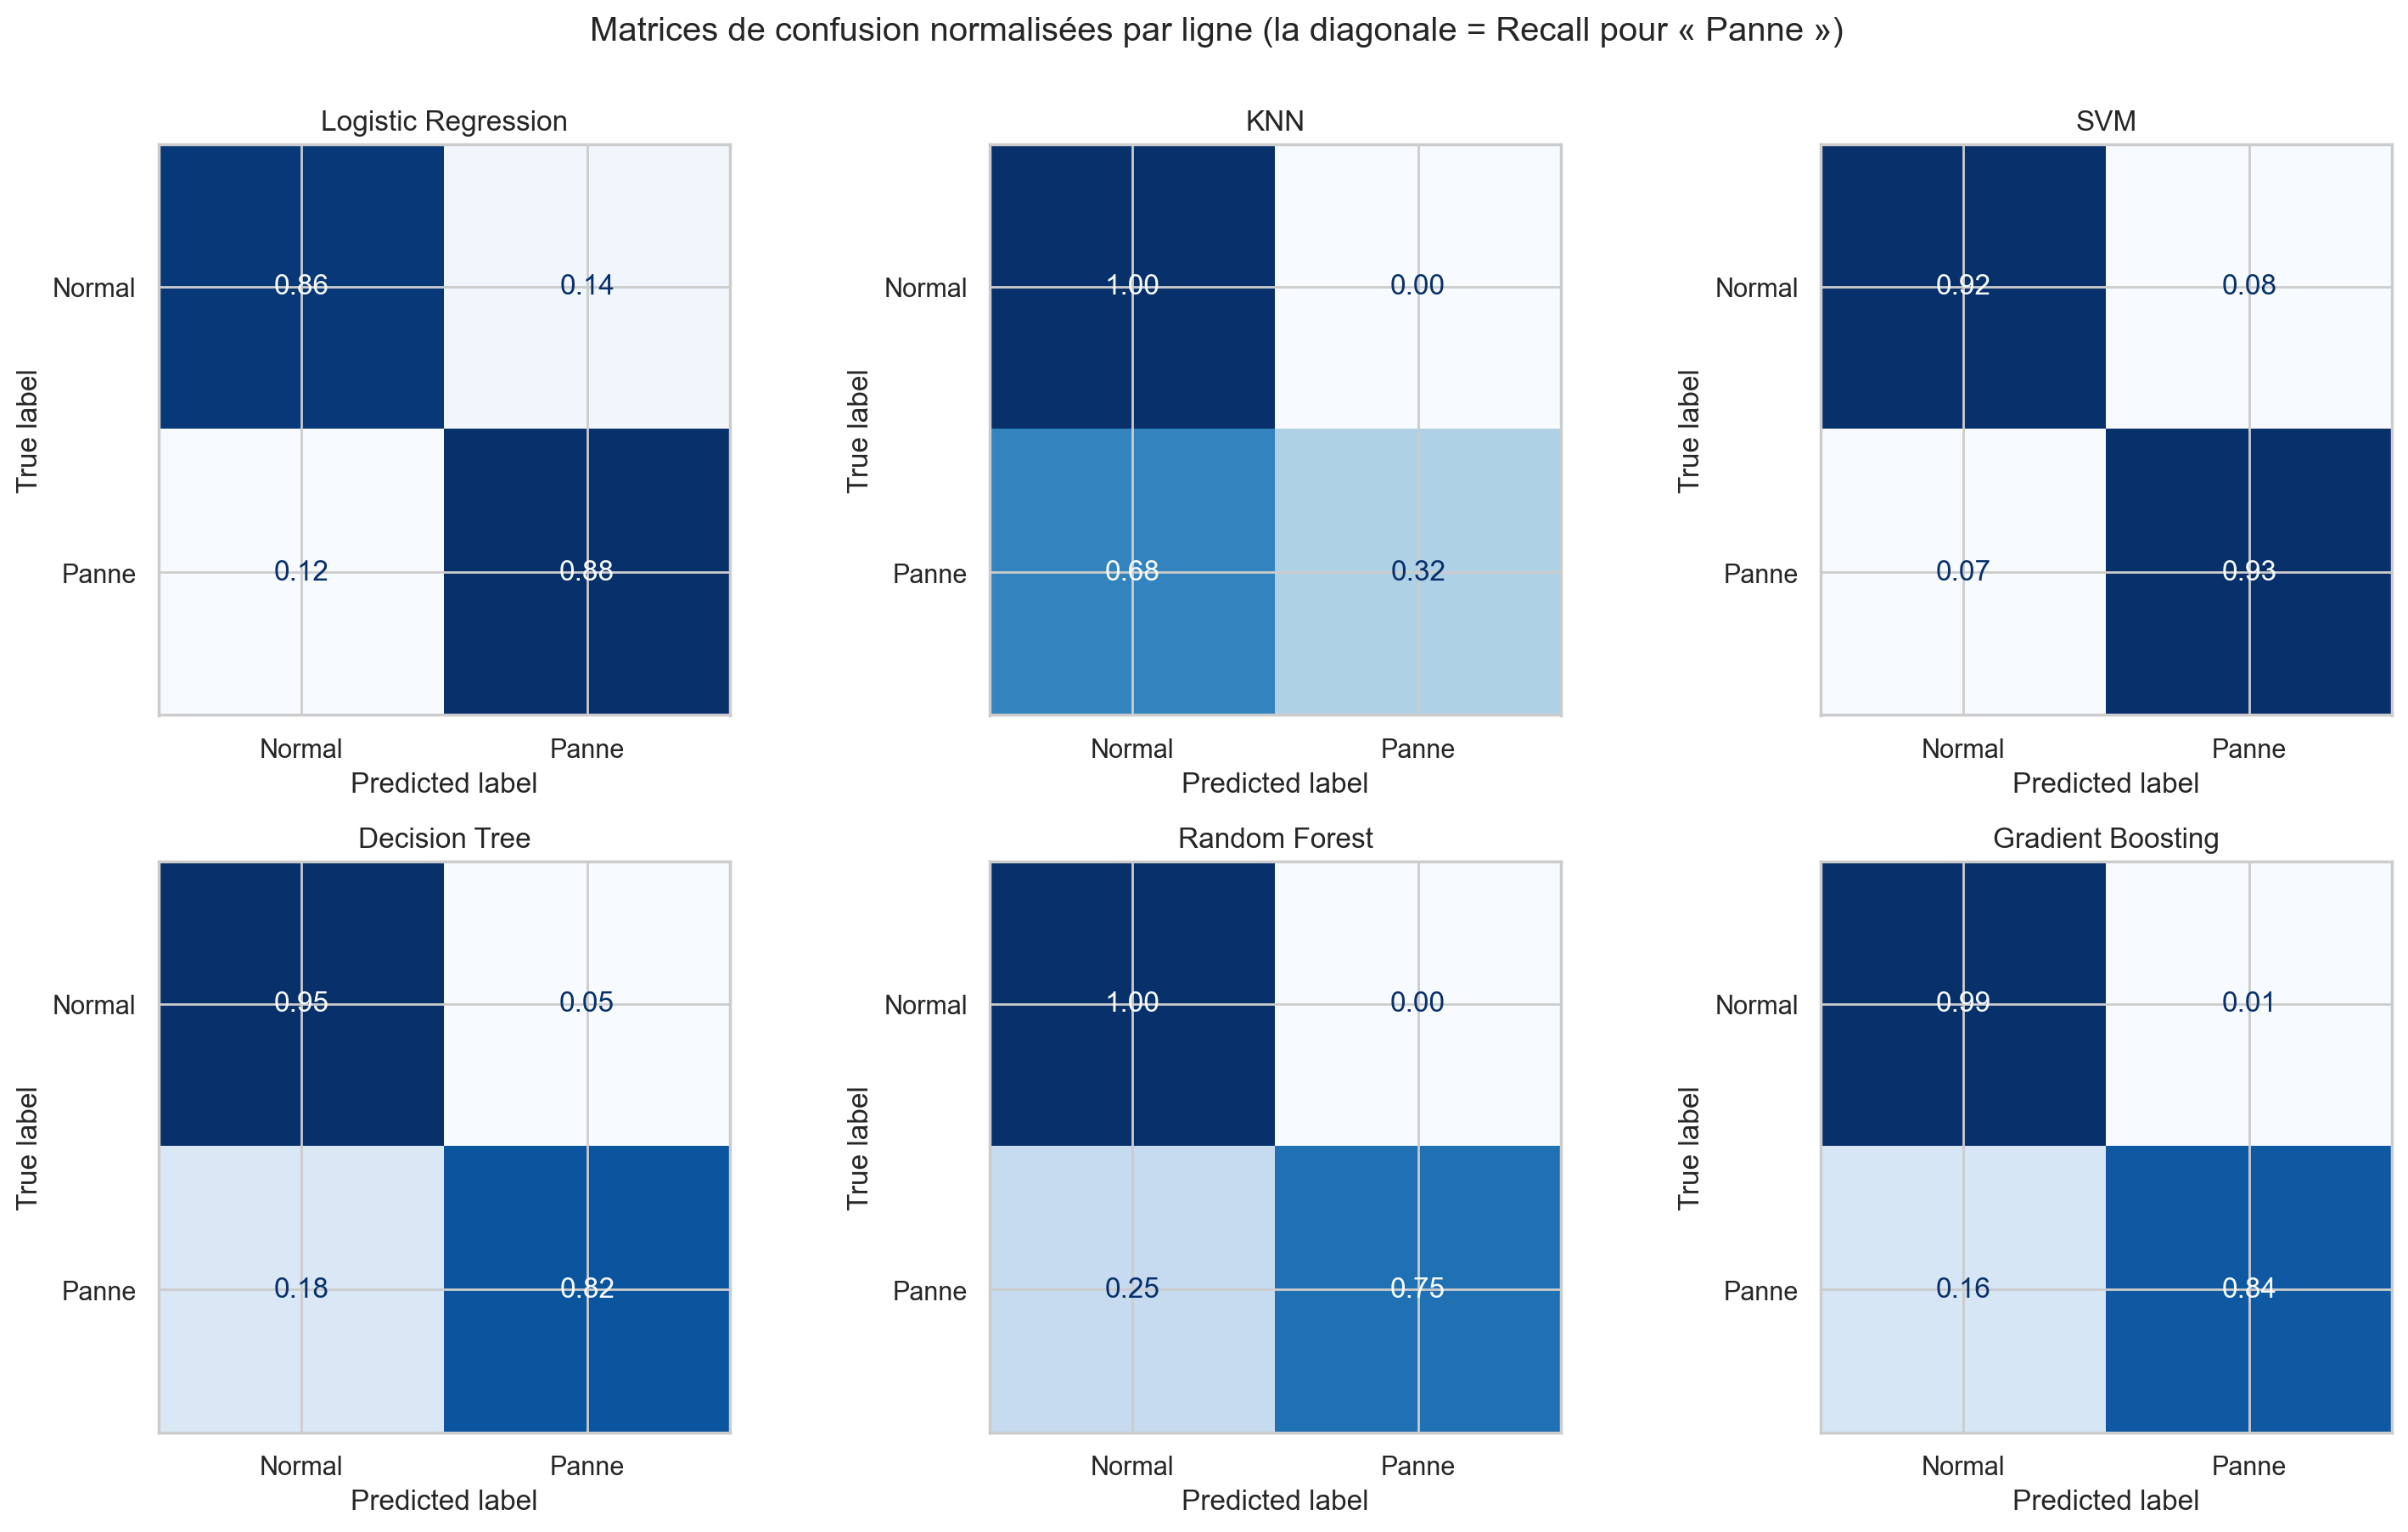
\includegraphics[width=0.82\textwidth]{figures/matrices_confusion.png}
  \caption{Matrices de confusion des modèles évalués sur le test.}
\end{figure}

% Exemple d'insertion de figure :
% \begin{figure}[H]
%   \centering
%   \includegraphics[width=0.9\textwidth]{figures/boxplots.png}
%   \caption{Boxplots des variables capteurs.}
% \end{figure}

\subsection{PCA}
\begin{table}[H]
\centering
\begin{tabular}{@{}lcc@{}}
\toprule
\textbf{Composante} & \textbf{Variance expliquée (\%)} & \textbf{Variance cumulée (\%)} \\
\midrule
PC1 & 33,44 & 33,44 \\
PC2 & 25,15 & 58,59 \\
PC3 & 19,29 & 77,88 \\
PC4 & 11,10 & 88,98 \\
PC5 & 8,19 & 97,17 \\
\bottomrule
\end{tabular}
\caption{Variance expliquée par les composantes principales.}
\end{table}

Nombre de composantes retenues pour 95\,\% de variance : 5. Les cinq composantes conservent 97,17\,\% de la variance ; PC1 et PC2 en représentent 58,6\,\%.

Les premières composantes combinent les variables thermiques et mécaniques. La projection PC1--PC2 fournit une vue synthétique utile, mais les pannes restent mélangées aux observations normales : les règles de panne sont des seuils et des interactions non linéaires que la PCA, transformation linéaire, ne sépare pas complètement.

\begin{figure}[H]
  \centering
  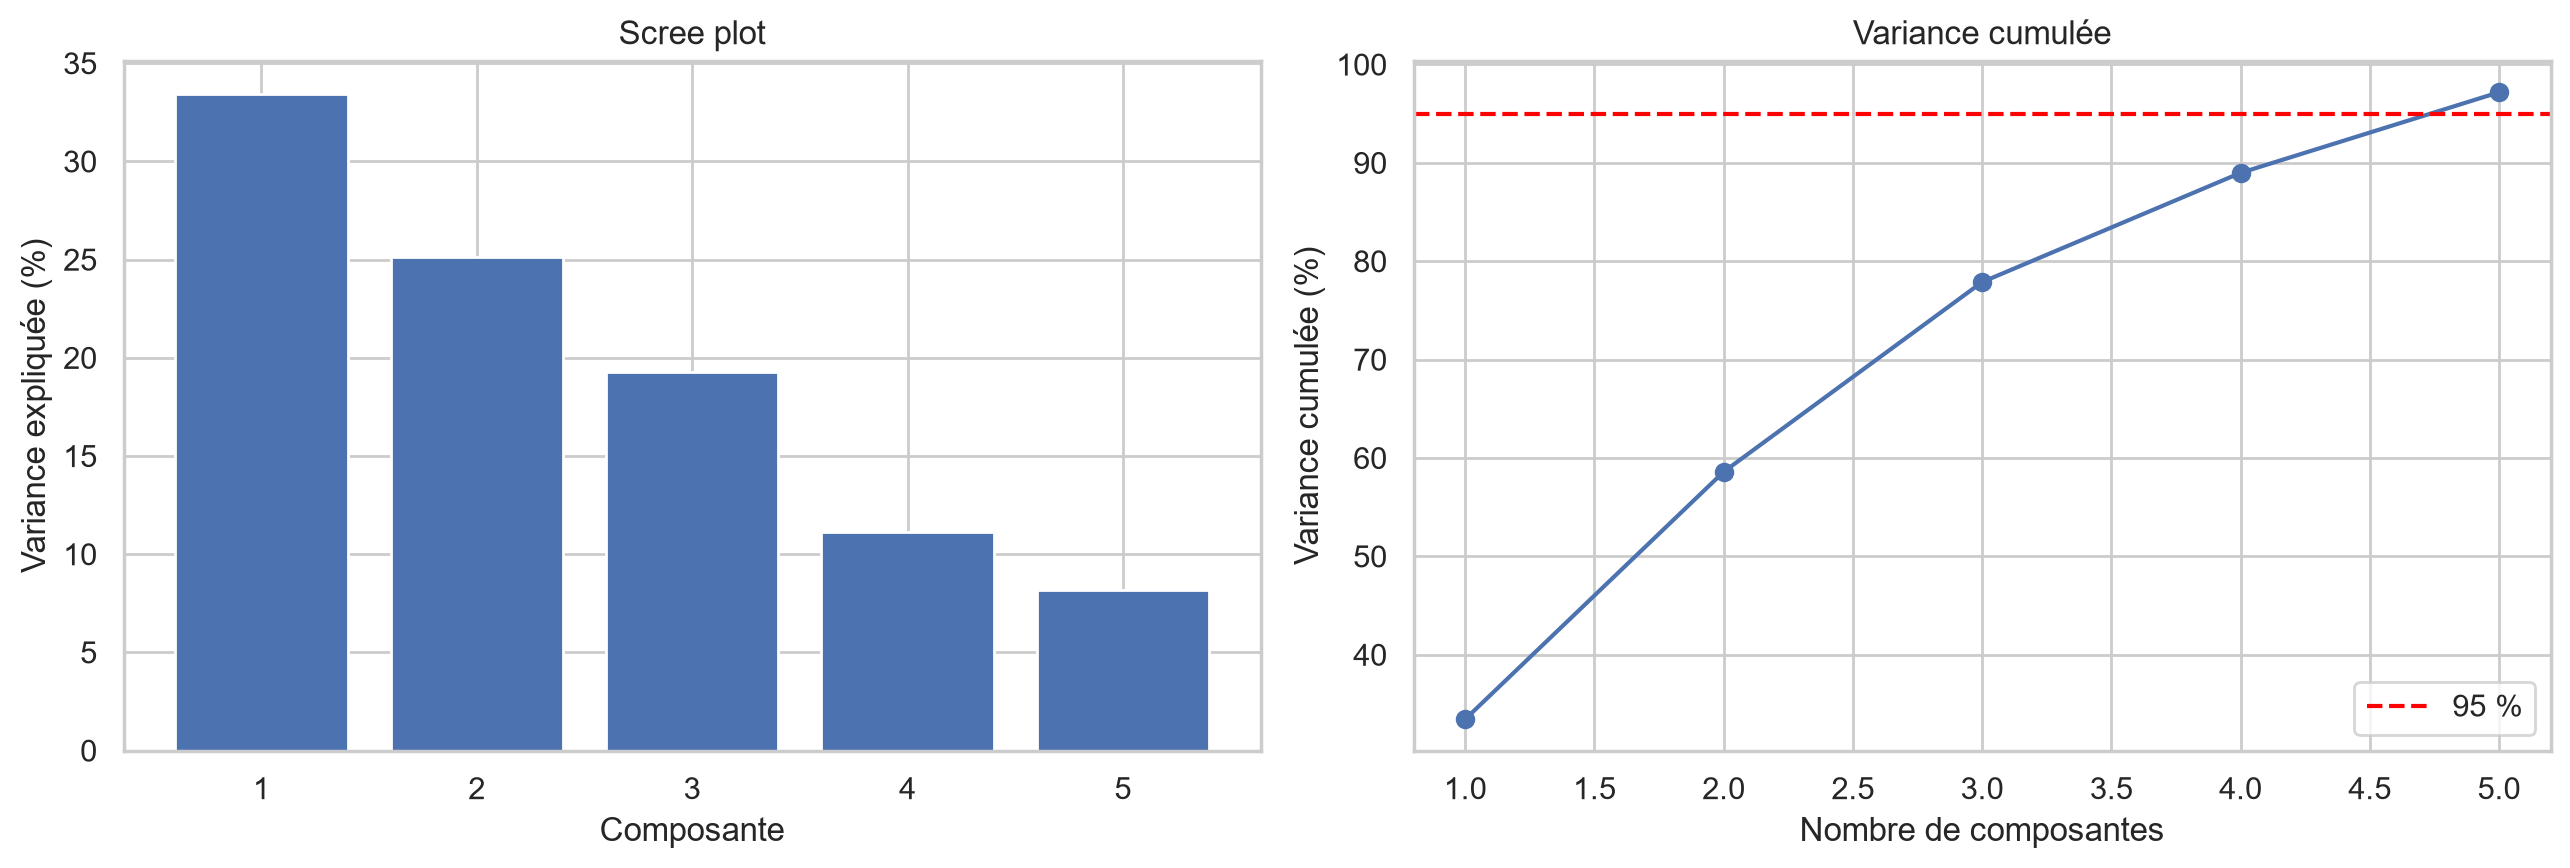
\includegraphics[width=0.92\textwidth]{figures/pca_variance.png}
  \caption{Variance expliquée individuellement et cumulée par la PCA.}
\end{figure}

\begin{figure}[H]
  \centering
  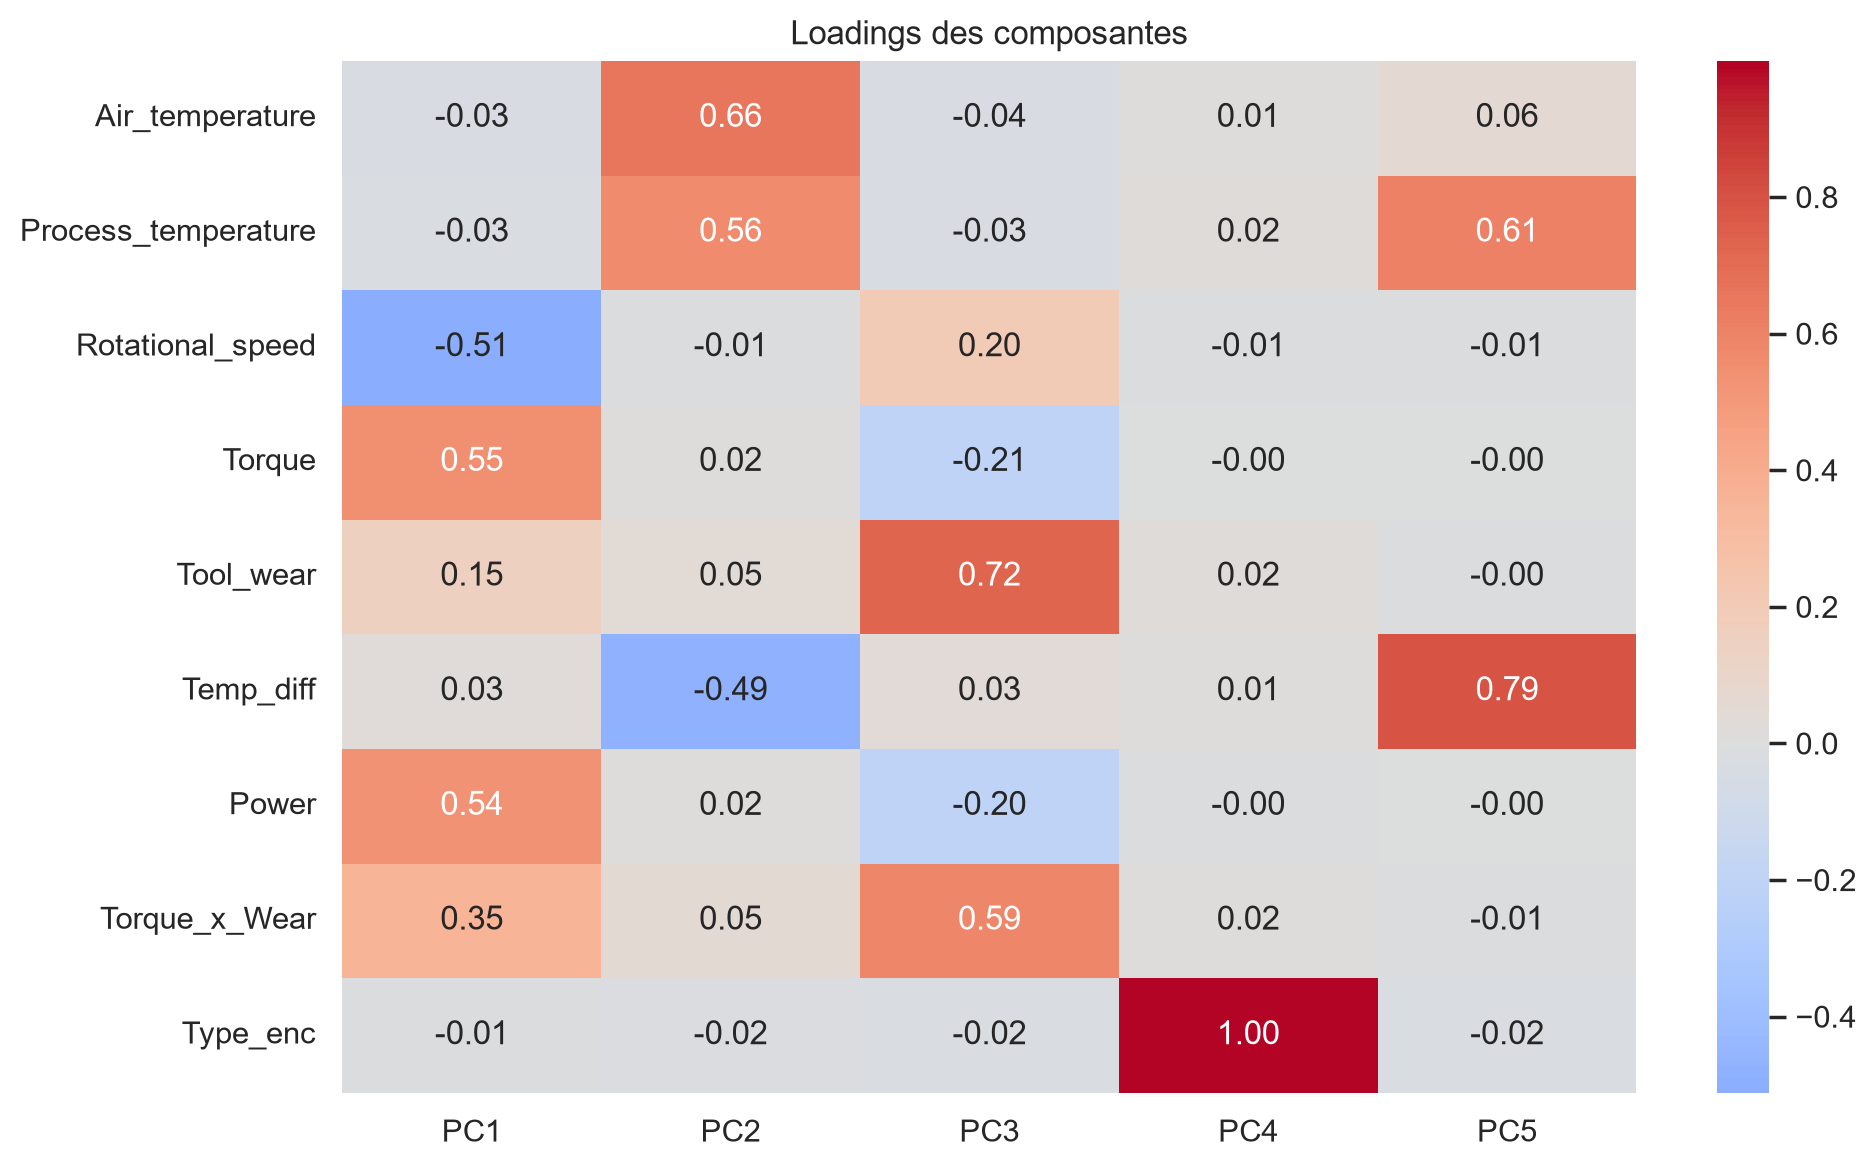
\includegraphics[width=0.88\textwidth]{figures/pca_loadings.png}
  \caption{Loadings des variables sur les composantes principales.}
\end{figure}

\subsection{K-Means}
Nombre de clusters retenu : $k = 4$, avec un score de silhouette de 0,2138 sur l'apprentissage. Le coude devient moins marqué après quatre groupes et la silhouette est maximale pour $k=4$ parmi les valeurs testées de 2 à 10.

\begin{table}[H]
\centering
\small
\begin{tabular}{@{}ccccl@{}}
\toprule
\textbf{Cluster} & \textbf{Nb machines} & \textbf{Nb pannes} & \textbf{Taux de pannes (\%)} & \textbf{Profil} \\
\midrule
0 & 2072 & 120 & 5,79 & Risque élevé \\
1 & 2134 & 98 & 4,59 & Risque élevé \\
2 & 2151 & 18 & 0,84 & Risque faible \\
3 & 1643 & 35 & 2,13 & Intermédiaire \\
\bottomrule
\end{tabular}
\caption{Clusters K-Means et taux de pannes.}
\end{table}

Le cluster 0 est le plus exposé : son taux de panne atteint 5,79\,\% sur l'apprentissage et 6,24\,\% sur le test, contre 3,4\,\% globalement. Il regroupe 44,3\,\% des pannes d'apprentissage et 47,1\,\% des pannes de test. K-Means identifie donc un groupe à risque, mais ne constitue pas à lui seul un classifieur de panne.

Détection d'anomalies par distance au centroïde :

\begin{table}[H]
\centering
\small
\begin{tabular}{@{}ccccc@{}}
\toprule
\textbf{Percentile} & \textbf{Machines signalées} & \textbf{Pannes détectées} & \textbf{Precision (\%)} & \textbf{Recall (\%)} \\
\midrule
90 & 210 & 34 & 16,19 & 50,00 \\
95 & 96 & 27 & 28,12 & 39,71 \\
99 & 14 & 10 & 71,43 & 14,71 \\
\bottomrule
\end{tabular}
\caption{Performance du détecteur d'anomalies par distance au centroïde (test).}
\end{table}

Le détecteur fait mieux que le hasard : même au percentile 90, la précision atteint 16,19\,\%, soit près de cinq fois le taux de base de 3,4\,%. Le percentile 99 fournit la meilleure précision (71,43\,%), mais au prix d'un recall faible (14,71\,%). Le choix du seuil dépend donc du coût relatif des fausses alertes et des pannes ratées.

\begin{figure}[H]
  \centering
  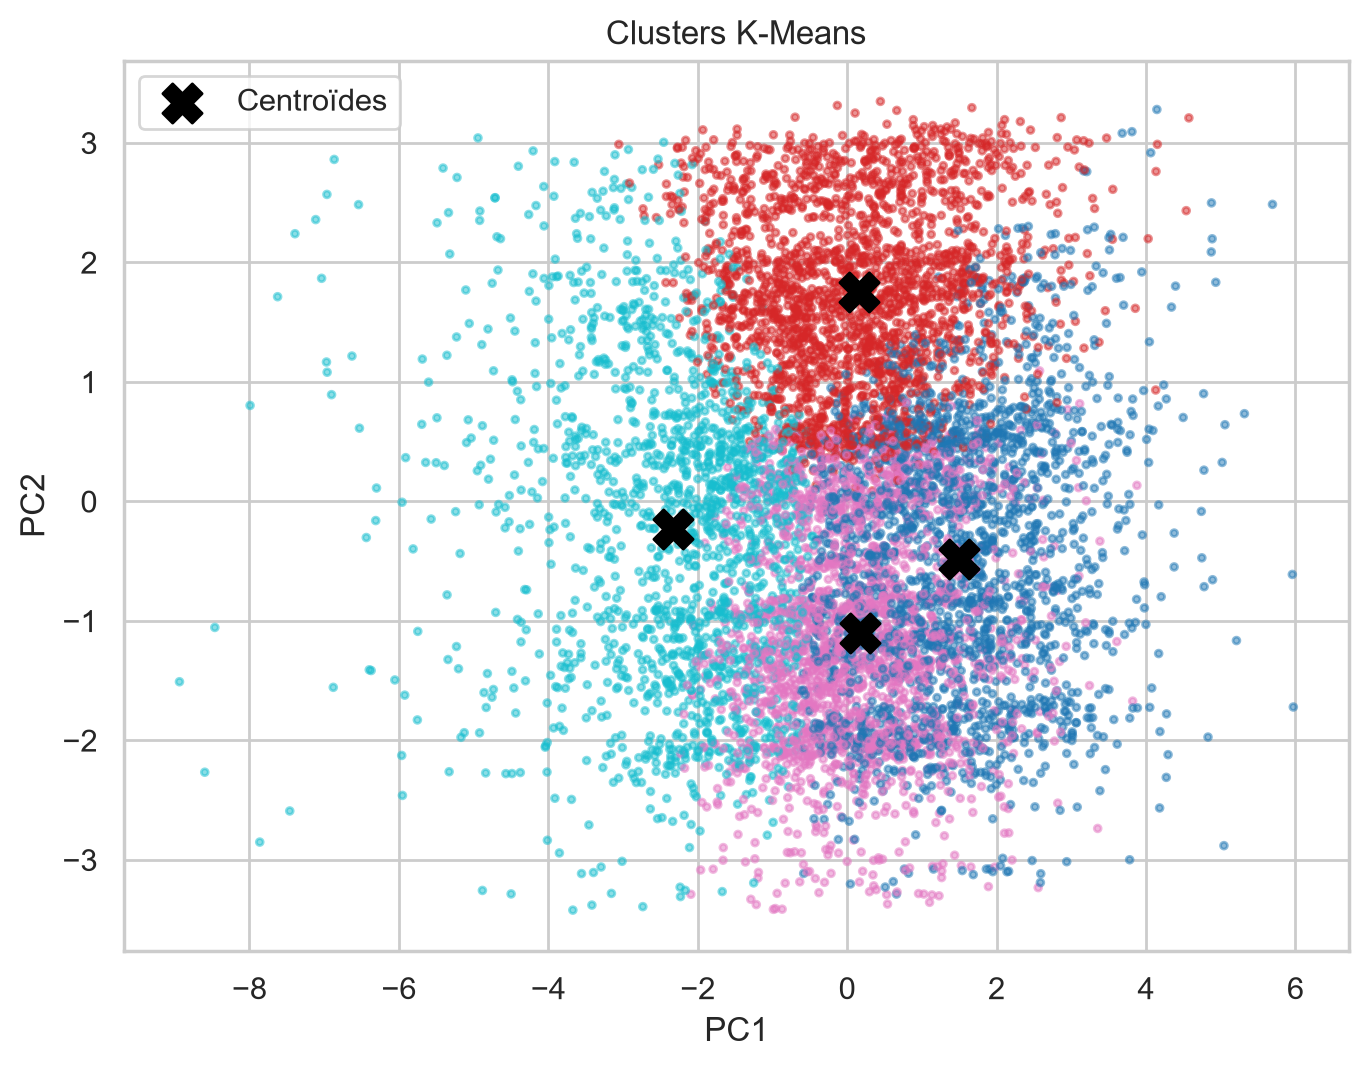
\includegraphics[width=0.86\textwidth]{figures/kmeans_clusters.png}
  \caption{Projection des clusters K-Means et de leurs centroïdes.}
\end{figure}

\section{Chapitre 6 — Modélisation et classification}\label{sec:classification}

\subsection{Classification : variables originales}
\begin{table}[H]
\centering
\scriptsize
\begin{tabular}{@{}lccccccc@{}}
\toprule
\textbf{Modèle} & \textbf{Acc.} & \textbf{Prec.} & \textbf{Recall} & \textbf{F1} & \textbf{ROC-AUC} & \textbf{PR-AUC} & \textbf{F1 (CV)} \\
\midrule
Régression logistique & 0,858 & 0,178 & 0,882 & 0,296 & 0,939 & 0,434 & 0,272 \\
KNN & 0,976 & 0,880 & 0,324 & 0,473 & 0,889 & 0,605 & 0,420 \\
SVM & 0,925 & 0,303 & 0,926 & 0,457 & 0,972 & 0,629 & 0,462 \\
Arbre de décision & 0,950 & 0,389 & 0,824 & 0,528 & 0,857 & 0,773 & 0,554 \\
Random Forest & 0,991 & 0,962 & 0,750 & 0,843 & 0,973 & 0,869 & 0,852 \\
Gradient Boosting & 0,990 & 0,851 & 0,838 & 0,844 & 0,976 & 0,893 & 0,846 \\
\bottomrule
\end{tabular}
\caption{Performances sur le test, variables originales.}
\end{table}

Sur les variables originales, le Gradient Boosting obtient le meilleur F1 de test (0,844), très légèrement devant le Random Forest (0,843), tandis que le Random Forest a le meilleur F1 moyen en validation croisée (0,852) et une PR-AUC CV de 0,889. Les écarts CV--test restent faibles pour ces deux modèles (0,009 et 0,002), ce qui ne suggère pas de sur-apprentissage marqué. Le SVM maximise le recall (0,926), mais génère 145 fausses alertes ; le Random Forest n'en génère que 2.

\subsection{Classification : composantes PCA}
Avec cinq composantes principales, les résultats de test sont : régression logistique (accuracy 0,718, precision 0,089, recall 0,794, F1 0,161, PR-AUC 0,187), KNN (0,973, 0,769, 0,294, 0,426, 0,535), SVM (0,904, 0,241, 0,853, 0,375, 0,478), arbre de décision (0,881, 0,191, 0,779, 0,307, 0,419), Random Forest (0,974, 0,711, 0,397, 0,509, 0,612) et Gradient Boosting (0,963, 0,471, 0,721, 0,570, 0,626). La PCA ne produit donc pas le meilleur classifieur.

\subsection{Comparaison variables originales et PCA}
La PCA dégrade le F1 et le recall de chacun des six modèles. La baisse de F1 est particulièrement forte pour le Random Forest (0,843 à 0,509) et le Gradient Boosting (0,844 à 0,570). La réduction est peu utile ici car le nombre de variables est déjà faible ; elle mélange en outre les capteurs et masque les seuils précis sur le couple, la vitesse et l'usure. Elle reste pertinente pour visualiser les données et faciliter l'exploration.

\begin{figure}[H]
  \centering
  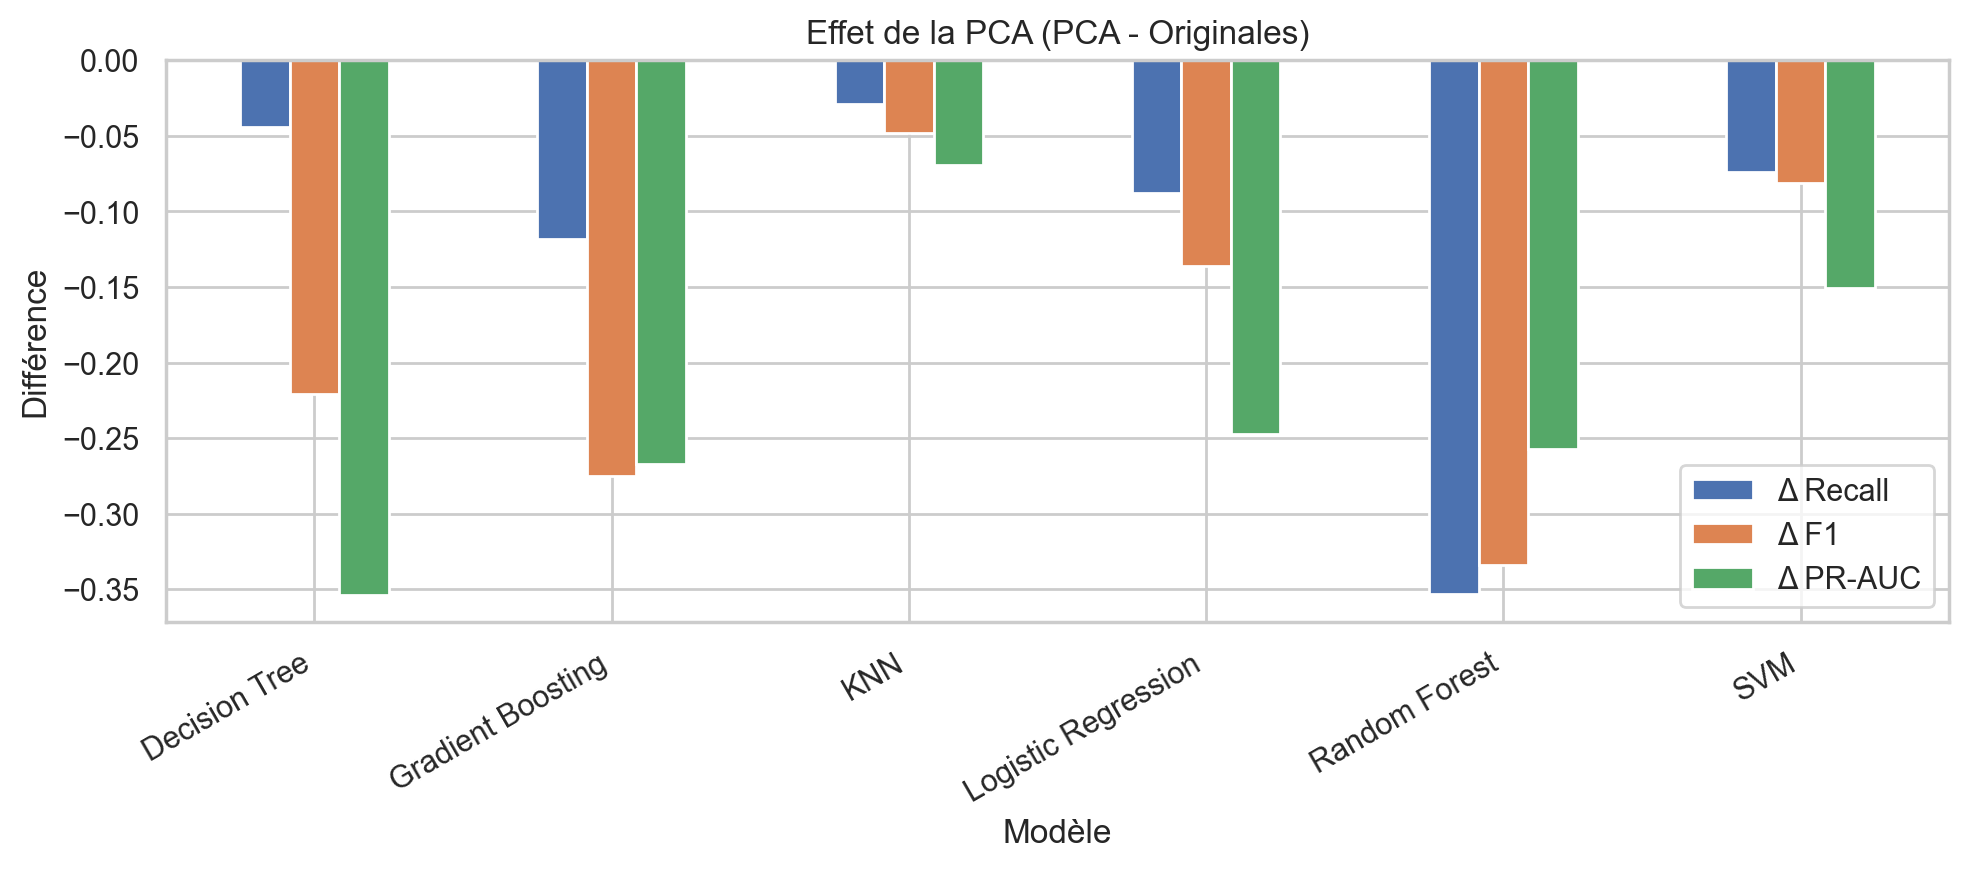
\includegraphics[width=0.88\textwidth]{figures/effet_pca.png}
  \caption{Effet de la PCA sur les performances des modèles.}
\end{figure}

\begin{figure}[H]
  \centering
  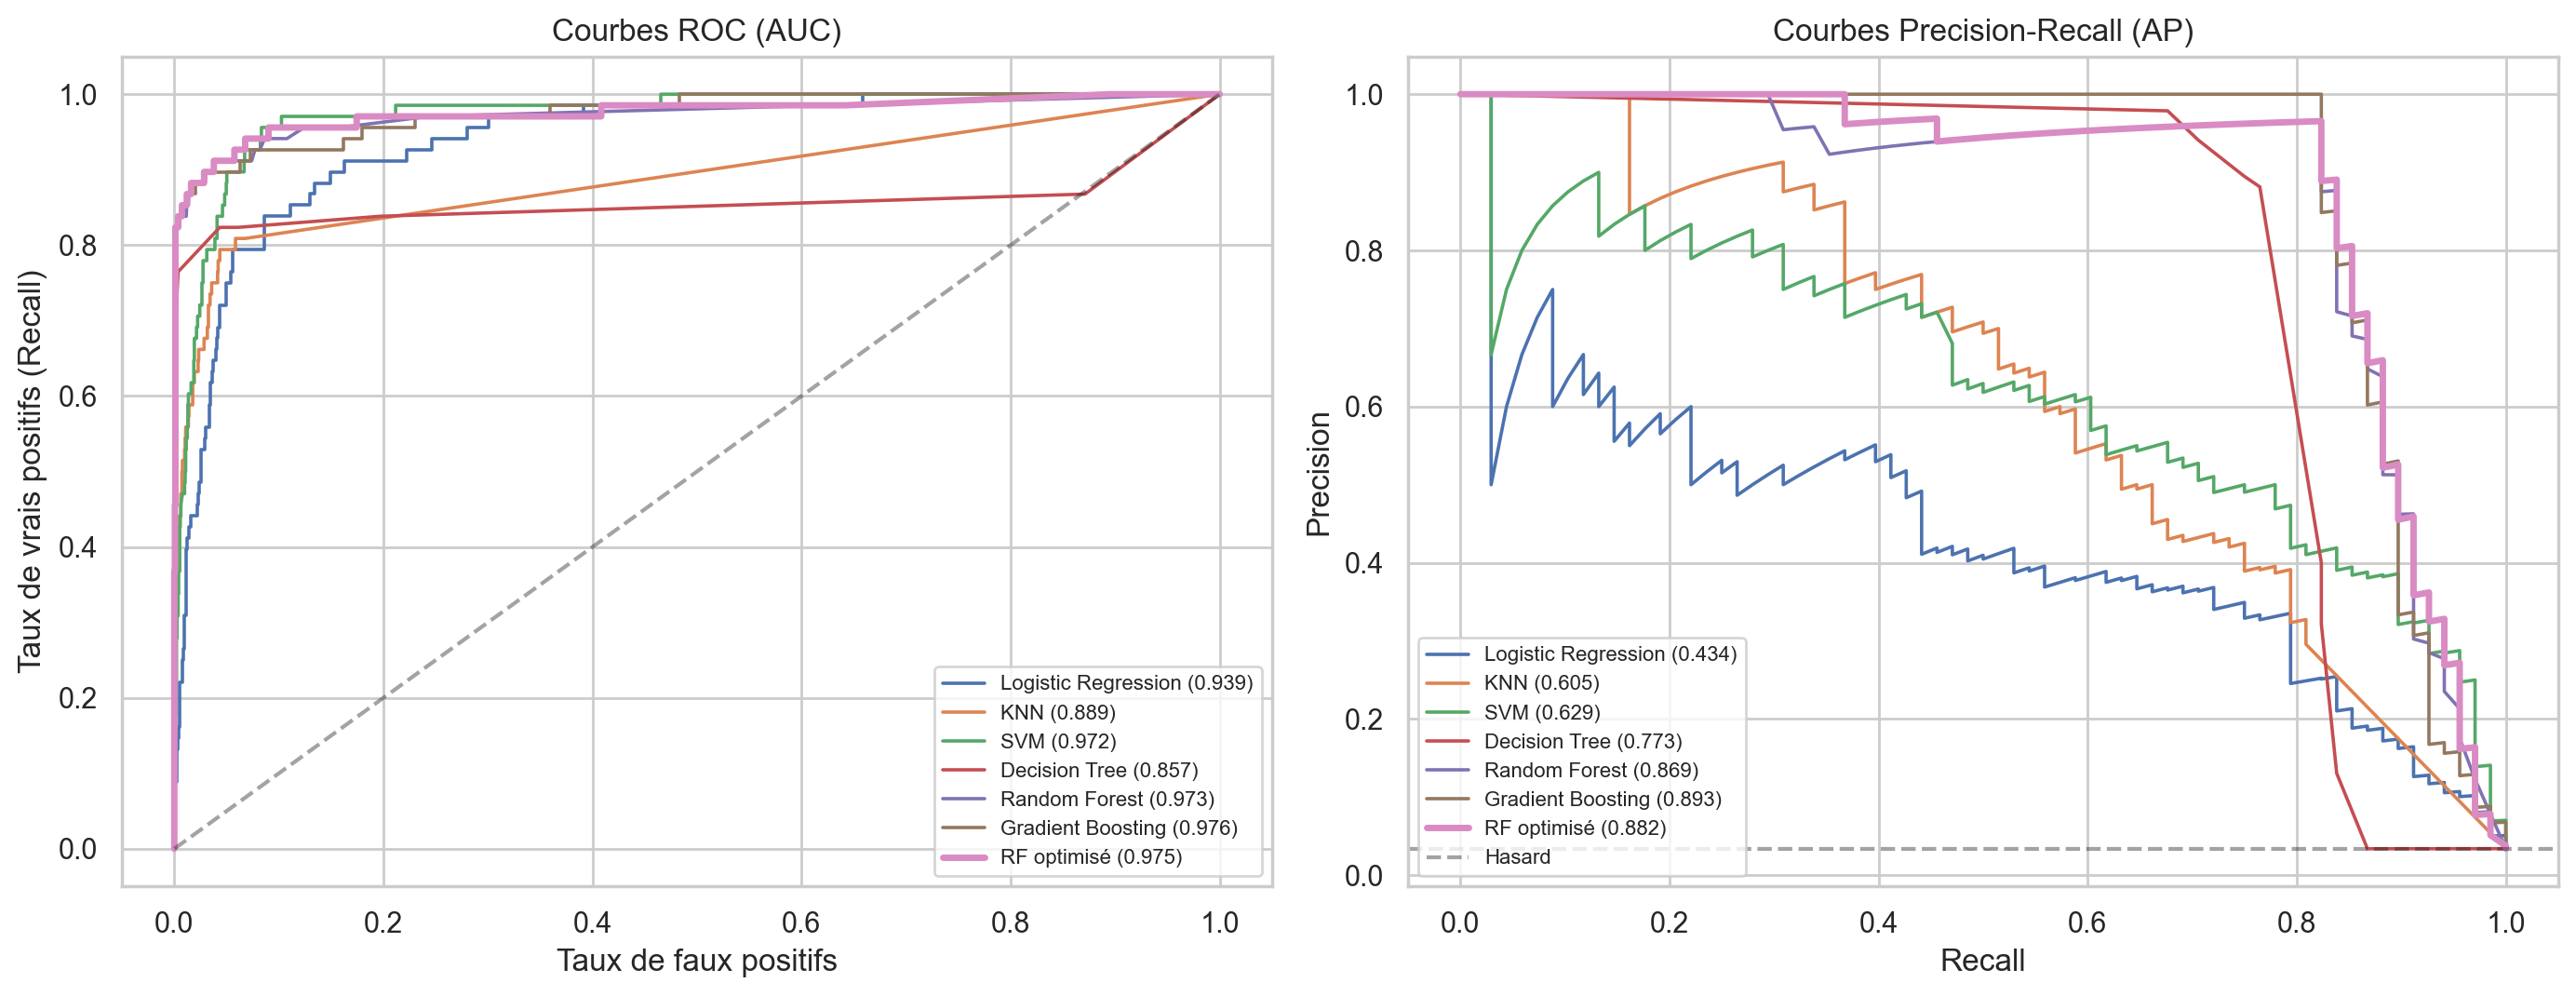
\includegraphics[width=0.9\textwidth]{figures/roc_pr.png}
  \caption{Courbes ROC et Precision--Recall sur le jeu de test.}
\end{figure}

\subsection{Optimisation et seuil de décision}
Meilleurs hyperparamètres du Random Forest : \texttt{n\_estimators=200}, \texttt{min\_samples\_split=2}, \texttt{min\_samples\_leaf=2}, \texttt{max\_features=0,5}, \texttt{max\_depth=10}. PR-AUC en validation croisée : 0,8997.

\begin{table}[H]
\centering
\begin{tabular}{@{}lcc@{}}
\toprule
\textbf{Métrique (test)} & \textbf{Seuil 0,5} & \textbf{Seuil ajusté (0,503)} \\
\midrule
Precision & 0,903 & 0,903 \\
Recall & 0,824 & 0,824 \\
F1 & 0,862 & 0,862 \\
\bottomrule
\end{tabular}
\caption{Effet de l'ajustement du seuil de décision.}
\end{table}

Le seuil optimal est très proche de 0,5 et conserve 56 vraies alertes, 12 pannes ratées et 6 fausses alertes. Le recall de 82,4\,% signifie qu'environ quatre pannes sur cinq sont détectées, tandis que la précision de 90,3\,% limite les inspections inutiles. En pratique, un seuil inférieur pourrait être choisi si le coût d'une panne ratée est dominant ; par exemple, à 0,3 le recall monte à 88,2\,%, mais la précision tombe à 59,4\,%.

\section{Chapitre 7 — Interprétation des résultats}\label{sec:interpretation}
\subsection{Importance des variables}
La vitesse de rotation est première selon l'importance MDI (0,241), suivie du couple (0,186), de la puissance (0,183) et de l'usure (0,160). En permutation, la vitesse reste première, suivie de \texttt{Temp\_diff} et de \texttt{Torque\_x\_Wear}. Les groupes mécanique, thermique et usure provoquent respectivement une baisse de PR-AUC de 0,743, 0,485 et 0,260. Ces résultats sont cohérents avec les mécanismes physiques étudiés.

\begin{figure}[H]
  \centering
  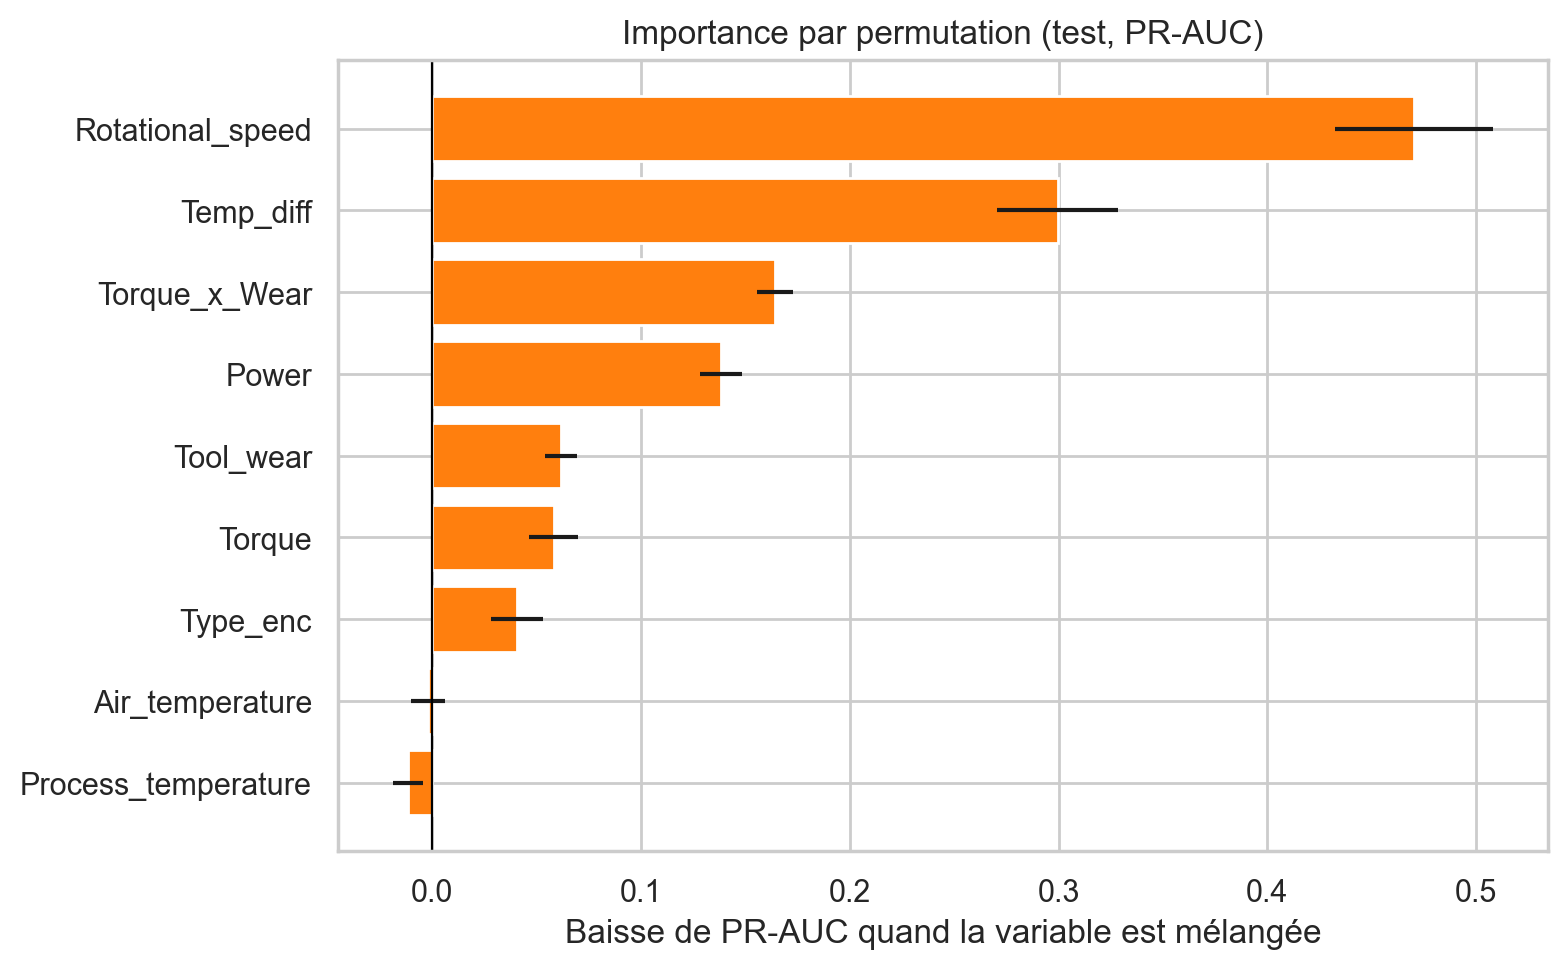
\includegraphics[width=0.82\textwidth]{figures/importance_permutation.png}
  \caption{Importance des variables par permutation.}
\end{figure}

\subsection{Performance par mode de panne}
L'évaluation par mode, disponible dans \texttt{evaluation\_par\_mode.csv}, montre une
forte hétérogénéité : le recall atteint 96,6\,\% pour HDF et 100\,\% pour PWF et
OSF, mais seulement 10\,\% pour TWF et 0\,\% pour RNF. Ces résultats doivent être
interprétés avec prudence, car certains modes ne comportent que quatre à dix
occurrences dans le test. Le modèle binaire ne réalise pas une classification
multi-classe des modes ; cette analyse décrit les recouvrements observés a posteriori.

\begin{figure}[H]
  \centering
  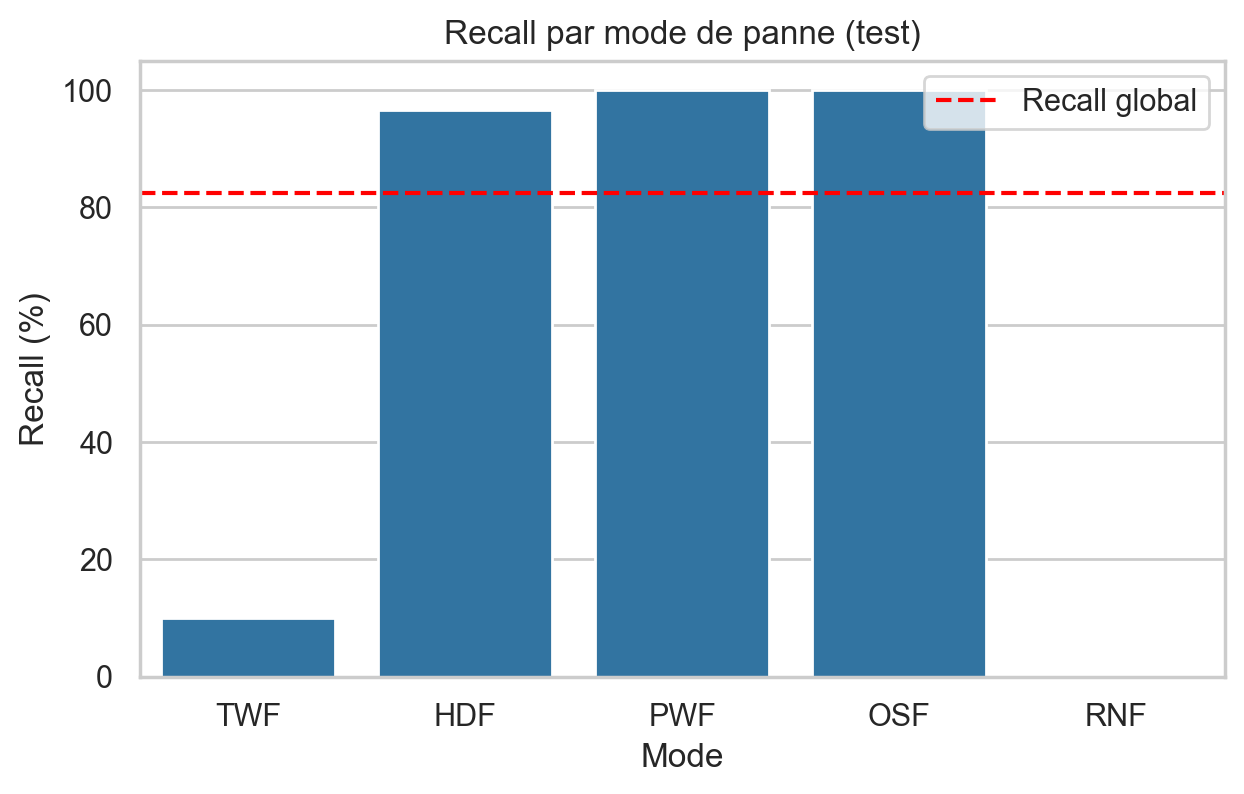
\includegraphics[width=0.82\textwidth]{figures/recall_par_mode.png}
  \caption{Recall du modèle optimisé selon le mode de panne.}
\end{figure}

% =====================================================
\section{Chapitre 8 — Conception et réalisation du tableau de bord}\label{sec:app}

\subsection{Architecture et chaîne de données}
Le dashboard est une application monolithique Streamlit définie dans
\texttt{app.py}. Les données tabulaires sont lues depuis \texttt{data/} avec
Pandas et les artefacts sérialisés depuis \texttt{models/} avec Joblib. Le
prétraitement du fichier importé reprend l'encodage du type et les trois variables
dérivées ; le scaler, la PCA et K-Means sauvegardés sont ensuite réutilisés pour
garantir la cohérence avec l'entraînement. Les fonctions de chargement utilisent
\texttt{st.cache\_data} et \texttt{st.cache\_resource}.

\subsection{Navigation et fonctionnalités}
La navigation comporte sept pages : Accueil, Capteurs, PCA, K-Means, Modèles,
Prédiction et Interprétation. L'Accueil expose les KPI du jeu actif, son aperçu
et la répartition Normal/Panne. Capteurs fournit un filtre par type puis des
histogrammes, boxplots, nuages de points, corrélations et statistiques.

La page PCA présente le scree plot, la variance cumulée, une projection 2D ou 3D
et la heatmap des loadings. K-Means affiche la taille et le taux de panne des
clusters, leurs profils normalisés, une projection PCA et un seuil de distance
réglable par percentile. La page Modèles compare le fichier de résultats et
recalcule, pour un modèle et un seuil choisis, les métriques et les courbes ROC
et Precision--Recall.

\subsection{Simulation d'une prédiction}
Prédiction permet une saisie manuelle ou cinq scénarios pédagogiques (machine
normale, usure, dissipation thermique, puissance et surcharge). La page calcule
les variables dérivées, affiche une probabilité de panne, applique un seuil
choisi, puis indique le cluster K-Means, la distance au centroïde et des repères
physiques issus du dataset. Les règles affichées sont des repères documentaires ;
elles ne remplacent pas le modèle.

\subsection{Interprétation et limites de l'interface}
Interprétation expose l'importance MDI, calcule à la demande l'importance par
permutation et affiche l'importance par groupes ainsi que les figures présentes.
Le fichier \texttt{shap\_summary.png} n'est pas présent : aucune analyse SHAP
n'est donc présentée comme disponible. Aucune capture d'écran du dashboard n'est
présente dans le dépôt ; le rapport décrit exclusivement les composants observés
dans le code. L'import d'un CSV est prévu, avec validation des colonnes et cible
facultative, mais ne constitue pas une ingestion temps réel.

\begin{figure}[H]
  \centering
  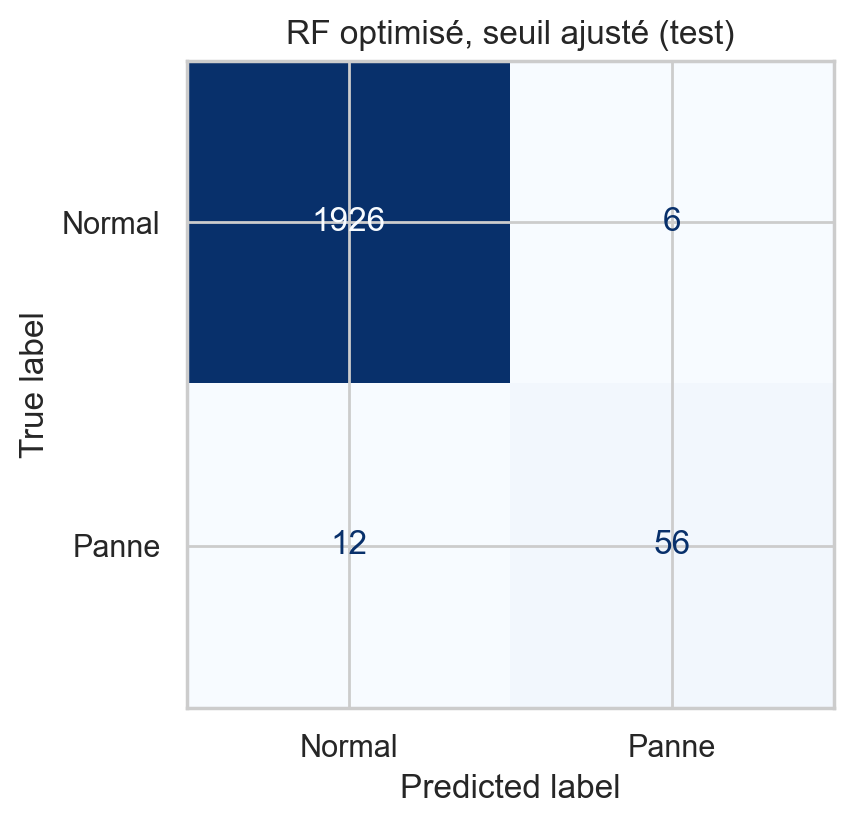
\includegraphics[width=0.82\textwidth]{figures/confusion_finale.png}
  \caption{Évaluation finale du Random Forest optimisé.}
\end{figure}

% =====================================================
\section{Chapitre 9 — Discussion générale, limites et perspectives}\label{sec:discussion}

\paragraph{Apport des variables construites.} Les variables \texttt{Temp\_diff}, \texttt{Power} et \texttt{Torque\_x\_Wear} traduisent les règles physiques qui génèrent les pannes. Elles occupent respectivement les rangs MDI 6, 3 et 5 ; avec \texttt{Type\_enc}, elles portent 36,1\,\% de l'importance totale.

\paragraph{Modèles à arbres.} Les résultats confirment cette hypothèse : Random Forest et Gradient Boosting obtiennent les meilleurs F1 et PR-AUC sur les variables originales. Les modèles linéaires conservent un recall élevé mais paient ce choix par beaucoup de fausses alertes.

\paragraph{Rôle de la PCA et de K-Means.} La PCA résume efficacement la variance pour l'exploration, mais dégrade la classification. K-Means détecte un cluster à risque et un score d'anomalie utile pour prioriser les inspections, sans remplacer le modèle supervisé.

\paragraph{Compromis precision/recall.} En maintenance, le coût d'une panne imprévue dépasse généralement celui d'une inspection inutile : on privilégie donc un recall élevé, quitte à accepter davantage de fausses alertes.

\subsection{Limites}
\begin{itemize}[noitemsep]
  \item Les données sont synthétiques : les performances ne se transposent pas directement à une usine réelle.
  \item Aucune dimension temporelle : chaque ligne est traitée indépendamment, sans historique de la machine.
  \item Peu de variables, et absence de capteurs de vibration, de pression, de tension et de courant.
  \item Nombre limité de pannes (environ 340), ce qui rend les estimations de recall sensibles à l'échantillonnage.
\end{itemize}

\subsection{Perspectives}
\begin{itemize}[noitemsep]
  \item Tester SMOTE ou d'autres techniques de rééchantillonnage, ainsi que XGBoost ou LightGBM.
  \item Classification multi-classes des modes de panne (TWF, HDF, PWF, OSF).
  \item Valeurs SHAP pour une interprétation locale de chaque prédiction.
  \item Validation sur des données réelles de capteurs, avec une dimension temporelle (séries temporelles, prédiction de la durée de vie restante).
  \item Déploiement avec surveillance en temps réel.
\end{itemize}

% =====================================================
\section{Chapitre 10 — Conclusion générale et perspectives}\label{sec:conclusion}
\section*{Conclusion synthétique}
\addcontentsline{toc}{section}{Conclusion}
Ce projet a mis en œuvre une chaîne complète de maintenance prédictive : préparation rigoureuse des données, exploration par PCA et K-Means, puis comparaison de six algorithmes avec des métriques adaptées au déséquilibre. Le Random Forest optimisé fournit le meilleur compromis opérationnel, avec une précision de 0,903, un recall de 0,824, un F1 de 0,862 et une PR-AUC de 0,882 sur le test. La PCA conserve 97,17\,\% de la variance mais dégrade les performances car elle masque les seuils et interactions physiques ; elle reste donc un outil de visualisation. La vitesse de rotation, le couple, la puissance, l'usure et l'écart de température sont les facteurs les plus associés aux pannes. Enfin, l'application Streamlit rend le pipeline accessible pour l'exploration et la simulation de nouvelles machines, tout en rappelant que la validation sur des données industrielles réelles reste indispensable.

% =====================================================
\begin{thebibliography}{9}
\bibitem{matzka2020} Matzka, S. (2020). \emph{Explainable Artificial Intelligence for Predictive Maintenance Applications}. Third International Conference on Artificial Intelligence for Industries (AI4I 2020).
\bibitem{uci} UCI Machine Learning Repository. \emph{AI4I 2020 Predictive Maintenance Dataset}. \url{https://archive.ics.uci.edu/dataset/601/ai4i+2020+predictive+maintenance+dataset}.
\bibitem{sklearn} Pedregosa, F. et al. (2011). Scikit-learn: Machine Learning in Python. \emph{Journal of Machine Learning Research}, 12, 2825--2830. \url{https://jmlr.org/papers/v12/pedregosa11a.html}.
\bibitem{streamlit} Streamlit Documentation. \url{https://docs.streamlit.io}.
\end{thebibliography}

\appendix
\section{Structure du projet}
\begin{table}[H]
\centering
\small
\begin{tabularx}{\textwidth}{@{}l X@{}}
\toprule
\textbf{Fichier} & \textbf{Contenu} \\
\midrule
\texttt{01\_pretraitement\_eda.ipynb} & Prétraitement, feature engineering, analyse exploratoire \\
\texttt{02\_pca.ipynb} & PCA, variance expliquée, projections \\
\texttt{03\_kmeans.ipynb} & K-Means, clusters, détection d'anomalies \\
\texttt{04\_classification.ipynb} & Six modèles, comparaison avec et sans PCA, seuil \\
\texttt{app.py} & Application Streamlit \\
\bottomrule
\end{tabularx}
\end{table}

\end{document}